\chapter{Introduction} % Depth 0

\begin{itemize}
\item \textred{Télécommunication} : Transmission d'information sous la forme de signaux électriques, sur un canal de communication
\item \textred{Signal} : Évolution d'une tension en fonction du temps
\end{itemize}

\section{Canaux de communications} % Depth 1

Deux types de canaux de communication : filaires (ligne téléphoniques, câbles coaxial, ...) et sans fils (ondes électromagnétiques).\\
Trois éléments caractérisent ces noyaux :
\begin{itemize}
\item \textred{L'Atténuation} (ou affaiblissement) : la diminution de l'amplitude ou de la puissance d'une onde ou d'un signal lors de sa transmission. Il augmente avec la distance.
\item \textred{Le Bruit} : partie du signal transmis dont on ne peut pas tirer d'information.
\item \textred{La Distorsion} ou \textred{dispersion} : l'ensemble des modifications indésirables d'un signal. Il y a plusieurs sources de distorsion :
	\begin{itemize}
	\item \textred{Les multitrajets} : Certains signaux arrivent directement à la source tandis que d'autres rebondissent sur des obstacles (par exemple des bâtiments). Par conséquent, le signal en arrivée est découpé en plusieurs morceaux de moindre intensité étalés sur le temps.
	\item \textred{L'effet Doppler} : La fréquence des signaux s'approchant de nous est différente de celle s'éloignant de nous
	\end{itemize}
\end{itemize}

L'information est représentée dans la forme du signal. Cela implique que changer l'amplitude du signal ne change pas l'information. En revanche lors de la distorsion du signal, celui-ci change de forme et il y a donc modification (ou perte) d'information.

En télécommunication, ce qu'on envoi sera toujours un signal analogique. Si on souhaite envoyer un signal numérique, il faut s'arranger pour le transposer en un signal analogique.

Il existe deux moyens de représenter les informations par des signaux : signaux analogiques ou signaux numériques (valeurs binaires). Une troisième technique est la \textred{numérisation} qui est la transformation de signaux analogiques en signaux numériques.

\section{Transformée de Fourier}

La transformée de Fourier est un moyen de représenter un signal par un ensemble de fréquences. La transformation de Fourier permet d'analyser tout signal en une somme de sinusoïdes (contenu fréquentiel).
\begin{align*} 
f(t) &\Leftrightarrow F(\omega)\\
F(\omega) &= \int_{-\inf}^{+\inf} f(t) e^{-j \omega t} dt\\
f(t) &= \frac{1}{2 \pi} \int_{-\inf}^{+\inf} F(\omega) e^{j \omega t} d\omega
\end{align*} 

\section{Modulation}

Les différents systèmes de télécommunication utilisent des bandes de fréquences bien précises pour chaque tâches. La modulation permet de transposer un signal autour d'une fréquence définie. Cette technique est utilisée pour partager les différentes bandes de fréquences.

Un \textred{signal modulé} est un \textblue{signal modulant} mis sur une \textblue{porteuse} à la fréquence désirée.

Le \textred{multiplexage} permet de faire passer plusieurs informations sur un seul support de fréquence. Les différents symboles sont combinés grâce à un multiplexeur. Deux types de multiplexage : \textblue{temporel} et \textblue{fréquentiel}.

\section{Exemples : Radio et télévision}

\subsection{Radio}

Avec la radio, les sons gauche ($G$) et droit ($D$) sont envoyés ensemble sous un signal $S_1 = G + D$ de façon à ce que les radios puissent le recevoir. Un autre signal est envoyé pour la stéréo : $S_2 = G -D$. Le signal stéréo peut être recréé par l'opération suivante :
\begin{align*}
G &= S_1 + S_2 = (G+D) + (D-G) = 2G\\
D &= S_1 - S_2 = (G+D) - (G-D) = 2D
\end{align*}

\subsection{Télévision}

Pour la télévision (analogique), le procédé est assez différent : la luminance (niveau de gris) des lignes est envoyé avec une pulsation de synchronisation (\textbf{synchronizing pulse}) entre chaque ligne.

Le canon à électrons utilisé dans les télévisions envoie la lumière ligne après ligne sur l'écran afin d'afficher une image. pour éviter certains effets désagréables, il est nécessaire que la fréquence à laquelle les images sont envoyées soit synchronisée avec celle du réseau électrique. En Europe, le débit d'image est donc de $50/s$ alors qu'aux USA et au Japon il est de $60/s$.

Une technique utilisée afin de réduire l'impression de scintillement sur les télévisions à tube cathodique et afin d'obtenir un meilleur débit d'images est l'entrelacement. Au lieu d'afficher l'image ligne par ligne, le canon envoie d'abord une ligne sur deux, en commençant par les lignes impaires. on utilise ainsi deux trames pour une image, soit un débit de 25 images par seconds (en Europe, 30 dans le reste du monde) au lieu de 50.

Pour l'envoi des couleurs, l'idée est la même que pour la radio : on va garder l'envoi de la luminance pour que les vieilles télévisions puissent toujours lire l'image et on va rajouter d'autres signaux afin de pourvoir avoir la couleur.

Soient $RGB$ les couleurs et $YUV$ les signaux (luminance $Y$ et chrominance $UV$) :
\begin{align*}
Y &= 0.3R + 0.59G + 0.11B\footnote{\text{Coefficient des couleurs : G>R>B, valeurs liées à la luminosité de chaque couleur}}\\
U &= 0.493(B- Y)\\
V &= 0.877(RY)
\end{align*}

De nos jours, la télévision numérique a remplacé la télévision analogique et les images sont désormais envoyées en binaire.

\section{Numérisation}

2 étapes : échantillonnage + quantification.

La \textred{numérisation} va permettre de passer d'un signal analogique à un signal numérique. on va pour \textblue{échantillonner} le signal (capturer des valeurs à intervalle fixe). Les avantages des signaux numériques sont :
\begin{itemize}
\item Le traitement et stockage de l'information
\item La régénération du signal par des codes correcteurs et détecteurs d'erreur.
\end{itemize}

Un signal analogique est représenté par des valeurs continues (ensemble $\mathbb{R}$) alors qu'un signal numérique est représenté par des valeurs discrètes (ensemble des chiffres représentables par des séries de 0 et de 1). Le procédé de transformation est appelé \textred{quantification} lors duquel on remplace les valeurs continues par des valeurs discrètes qui s'en rapprochent le plus.

L'un des gros avantages du numérique est que même s'il y a du bruit lors de la transmission de l'information, moyennant une faible distorsion, l'information retransmise sera parfaite car le bruit sera filtré et remplacé par une valeur binaire. Contrairement à l'analogique où le bruit est transmis et non filtré.

Il faut faire très attention lors de l'échantillonnage des erreurs possibles. En effet, choisir un intervalle de temps trop large pour capturer les valeurs peut causes des erreurs. Cependant si on le fait correctement, le \textit{théorème de Shannon} certifie qu'il n'y aura aucune perte d'information.

\textred{Théorème de Shannon} : La fréquence d'échantillonnage doit être au moins deux fois la fréquence maximum du signal.

\chapter{Lignes}

\section{Caractéristiques des lignes}

Trois éléments caractérisent une ligne :
\begin{enumerate}
\item L'atténuation
\item La distorsion
\item Le bruit
\end{enumerate}

Tous ces éléments dépendent de la géométrie, des matériaux et des conditions dans lesquelles ces lignes opèrent (il y a de nombreux types de lignes différents : ligne bifilaire, ligne coaxiale, fibre optique etc.).

\section{Modélisation d'une ligne}

On représente habituellement les lignes comme une résistance $R'(\Omega / m)$, une conductance $G''$, une inductance $L'$ et une capacité $C''$. Le morceau de ligne suivant se répète tout au long de la ligne :

\begin{figure}[H]
    \centering
    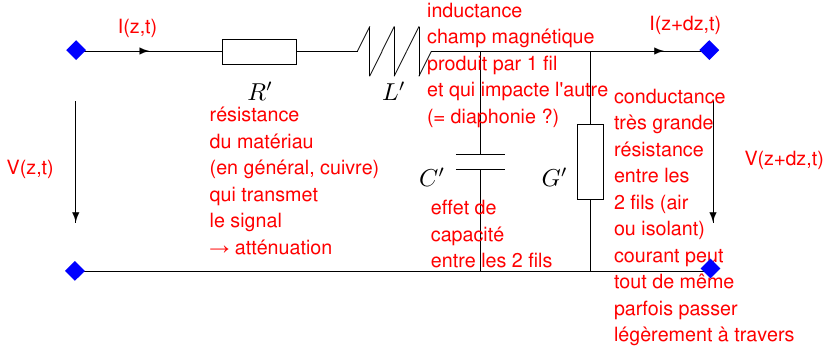
\includegraphics[width=0.7\textwidth,keepaspectratio]{ligne}
    \caption{Modélisation d'une ligne}
\end{figure}

Ces paramètres varient suivant le type de ligne, la fréquence et le matériel utilisé. L'équation des télégraphistes nous donne la relation suivante (avec $z$ la position, $t$ le temps et $v$ la tension sur la ligne :
\begin{equation*}
\frac{\partial^2v}{\partial z^2} = LC\frac{\partial^2v}{\partial t^2}+(RC+LG)\frac{\partial v}{\partial t}+RGv
\end{equation*}

Dans le cas d'un contexte où les pertes seraient négligeables ($R=G=0$) nous obtiendrons la formule suivante (équation des ondes) : 
\begin{equation*}
\frac{\partial^2v}{\partial z^2} = LC\frac{\partial^2v}{\partial t^2}
\end{equation*}

Qui fait le lien entre une variation de tension en fonction de la position et une variation de la tension en fonction du temps. Posons $c = \frac{1}{\sqrt{LC}}$ \footnote{Dans la plupart des lignes : $c \approx$ proche de la vitesse de la lumière} et nous avons la tension :
\begin{equation*}
v = f(z+ct) + g(z - ct)
\end{equation*}

Cette équation montre que l'on peut déplacer (propager) n'importe quelle combinaison de fonction vers la gauche ($g$) ou vers la droite ($f$)

\section{Effet pelliculaire}

L'\textred{effet pelliculaire} (ou l'effet de peau) est un effet électromagnétique qui repousse les lignes de courant vers la surface du conducteur. Les électrons vont donc s'amasser sur les bords.

Cet effet de peau va en fait diminuer la surface de la ligne qui est effectivement parcourue par du courant et donc augmenter la résistance de celui-ci. Il est causé par la création d'un champ magnétique.
\begin{equation*}
\nearrow \text{ fréquence } \Rightarrow \nearrow \text{ effet de peau } \Rightarrow \nearrow \text{ résistance } \Rightarrow \nearrow \text{ pertes }
\end{equation*}

En d'autres termes, cet effet est comparable au diamètre d'un tuyau (plus gros est le tuyau, plus gros est le débit). Ici, le courant dans la ligne ne passe pas au milieu et se concentre principalement sur les bords/la surface du conducteur donc l'espace est restreint ce qui entraîne moins de débit. Cet effet augmente avec la fréquence (basse fréquence : $\pm $ réparti, haute fréquence : concentré sur les bords).

\section{Atténuation}

L'\textred{atténuation d'un signal} d'une ligne peut être calculée comme étant $10 log(\frac{P_1}{P_2})$, avec $P_1$ la puissance d'entrée et $P_2$ la puissance de sortie. Cette atténuation se mesure en \textblue{décibels ($dB$)}.

On sait que $P=\frac{V^2}{R}$ donc $\frac{P_1}{P_2} = \frac{v_1^2}{v_2^2}$. Si on souhaite exprimer l'équation de l'atténuation sous forme de tensions, on a :
\begin{equation*}
10 log(\frac{P_1}{P_2}) = 10 log(\frac{v_1^2}{v_2^2}) = 20 log(\frac{v_1}{v_2})
\end{equation*}

\section{Dispersion}

Soient le nombre de pulsations $\omega = 2 \pi f$, le vecteur d'onde $\beta = \frac{2 \pi}{\lambda}$ et $\lambda$ la longueur d'onde, on a la vitesse de phase (vitesse propagation) :
\begin{equation*}
v_{ph} = \frac{\omega}{\beta}
\end{equation*}

la dispersion d'un signal provient des différent vitesses de déplacement des fréquences constituant une onde. L'onde à tendance à s'étaler sur le temps plus la ligne sera longue.

\section{Impédance caractéristique}

L'impédance permet de connaître le rapport tension/courant et est utile dans beaucoup de systèmes pour savoir quelle tension on va récupérer en envoyant un certain courant. L'impédance caractéristique ($Z_c$) désigne l'impédance en supposant une ligne infinie.

La loi d'ohm caractérise une tension $v$ en fonction d'une résistance $r$ (ou $z$ pour les résistances avec des nombres complexes) et d'un courant $i$ :
\begin{equation*}
v = ri \text{ ou } v = zi
\end{equation*}

$z$ est totalement réel pour une résistance pure et totalement imaginaire pour une inductance/capacité pure.

L'impédance d’une ligne en fonction de son impédance d’entrée $Z_{in}$ :
\begin{itemize}
\item Dans le cas d'une \textred{ligne infinie}, l'impédance d'entrée est égale à l'impédance caractéristique de la ligne $Z_{in} = Z_c$.
\item Si une ligne se termine sur une impédance $Z_c$ et que cette ligne est \textblue{adaptée}, elle ne présentera pas de réflexion et $Z_{in} = Z_c$.
\end{itemize}

Une \textblue{ligne adaptée} est un ligne se comportant comme une ligne infinie où l'impédance du récepteur est égale à $Z_c$ (impédance caractéristique de la ligne). Cela permet entre autre d'éviter la réflexion du signal.

\section{Exposant de propagation}

Il arrive qu'il y ait de la dispersion (déphasage) et de l'affaiblissement linéique (atténuation). Soient $\alpha$ l'\textblue{atténuation} et $\beta$ le \textblue{déphasage}, l'\textred{exposant de propagation} se calcul avec :
\begin{equation*}
\gamma = \sqrt{(R + j \omega L)(G + j \omega C)} = \alpha + j \beta
\end{equation*}

Habituellement, dans une ligne où $G$ est négligeable, deux cas se présentent :
\begin{itemize}
\item Cas $\omega L << R$ : Correspond au cas ù le fil a beaucoup de résistance. Mauvaise situation dans laquelle nous avons de la distorsion.
\item Cas $\omega L >> R$ : Correspond au cas où le fil a peu de résistance. Bonne situation dans laquelle il y a peu de distorsion car l'effet inductif de la ligne > l'effet résistif de la ligne.
\end{itemize}

\section{Pupinisation}

Pour le cas de lignes tel que $\omega L << R$, nous allons procéder à une \textred{pupinisation}.
Cela consiste à insérer des inductances le long de la ligne afin d'augmenter artificiellement $L$.
Grâce à cela nous allons avoir une réduction de l'atténuation le long de la ligne (filtre passe-bas).

Toutefois, la pupinisation n'est bénéfique que pour une certaine bande de fréquences car elle cause l'attén-\\uation des fréquences supérieures.
Puisque l'on a besoin de ces fréquences de nos jours, notamment pour l’ADSL, la pupinisation n’est donc plus utilisée.

\section{Lignes bifilaires}

Les lignes bifilaire sont des lignes de transmission constituées de \textblue{deux fils parallèles} séparés par un \textblue{isolant}. Elles sont souvent rassemblées dans des quartes torsadées (quatre fils ensemble) ou encore dans des bottes de quartes (50 fils). Il arrive par contre dans ce genre de groupements que nous trouvions de la \textblue{diaphonie}.

La \textred{diaphonie} (parfois \textblue{bruit} ou \textblue{crosstalk} en anglais) est l'interférence d'un premier signal avec un autre.

Avantages et inconvénients des lignes bifilaires:
\begin{itemize}
	\item[+] Faible coût
	\item[+] Connexions aisées
	\item[+] Pré-installation dans les bâtiments
	\item[+] Faible atténuation aux basses fréquences
	\item[-] Atténuation importante aux hautes fréquences (l'atténuation augmente fort avec la fréquence)
	\item[-] Rayonnement important (sensibilité aux interférences)
	\item[-] Problème de confidentialité
\end{itemize}

\subsection{Câble coaxial}

Un câble coaxial est constitué d'une \textblue{partie centrale} (fil de cuivre) enveloppé dans un \textblue{isolant}, puis d'un \textblue{blindage métallique} tressé et enfin d'une \textblue{gaine extérieure}. Il est utilisé comme câble pour la transmission de la télédistribution.

Avantages et inconvénients du câble coaxial :
\begin{itemize}
	\item[+] Large bande passante ($\sim 500 MHz$)
	\item[+] Protection contre les interférences grâce à la gaine extérieure
	\item[+] Technique éprouvée et répandue
	\item[+] Facilité de réparation et de connexion
	\item[+] Moins de résistance
	\item[+] Atténuation moindre
	\item[-] Fréquences limitées
	\item[-] Blindage jamais parfait
\end{itemize}

\subsection{Fibre optique}

Une fibre optique est un conducteur de lumière en \textblue{fil en verre ou en plastique} très fin utilisé pour la transmission de données (sous forme de lumière).

Un \textred{mode} est un chemin emprunté par la lumière par rapport à sa réflexion et réfraction au sein de la fibre optique.

\textred{Dispersion intermodale} : phénomène correspondant à l'existence de différentes vitesses possibles pour la propagation des ondes. La distance parcourue par certains modes est différentes de celle d'autre mode. Il y a donc une dispersion du signal. Ce n'est pas lié à la vitesse mais aux chemins plus ou moins long parcourus par les ondes

\textred{Transducteur} : dispositif convertissant un signal physique en un autre, par exemple un signal lumineux.

Avantages et inconvénients du câble coaxial :
\begin{itemize}
	\item[+] Énorme bande passante
	\item[+] Très faible atténuation
	\item[+] Immunité à l'égard des rayonnements
	\item[+] Isolation électrique
	\item[+] Encombrement, poids, coût faibles
	\item[-] Connexions difficiles
	\item[-] Réparations difficiles
	\item[-] Disponibilité de transducteurs
	\item[-] Technologie en développement
\end{itemize}

\subsubsection{La transmission dans une fibre optique}

Lorsqu'un rayon lumineux entre dans une fibre optique à l'une de ses extrémités avec un angle adéquat, il subit de multiples réflexions totales internes. Ce rayon se propage alors jusqu'à l'autre extrémité de la fibre optique sans perte, en empruntant un parcours en zigzag.

On s'assure que la différence entre l'indice de réfraction $n_1$ (largeur) et l'indice de réfraction $n_2$ (longueur) soit suffisamment grande pour que les rayons soient réfléchis et restent à l'intérieur.

\begin{figure}[H]
\begin{center}
\begin{tikzpicture}[line cap=round,line join=round,>=triangle 45,x=1.0cm,y=1.0cm]
	\clip(1.35,-0.01) rectangle (8.1,2.5);
	\draw [domain=1.4:8] plot(\x,{(--2.81-0*\x)/1.16});
	\draw [domain=1.4:8] plot(\x,{(-0-0*\x)/2.74});
	\draw (8,0) -- (8,2.41);
	\draw (1.4,0) -- (1.4,2.41);
	\draw (1.4,1.02)-- (3.12,2.42);
	\draw (3.12,2.42)-- (5,0);
	\draw (5,0)-- (6.86,2.42);
	\draw (6.86,2.42)-- (8,0.86);
	\draw (1.4,1.02)-- (3,0);
	\draw (3,0)-- (5.06,2.42);
	\draw (5.06,2.42)-- (7,0);
	\draw (7,0)-- (8,1.66);
	\draw (1.4,1.02)-- (8,1.18);
	\draw (1.4,1.02)-- (4,0);
	\draw (4,0)-- (8,2);
	\draw (1.4,1.02)-- (4.14,2.42);
	\draw (4.14,2.42)-- (8,0.42);
	\draw (8,0.42)-- (8,2);
	\draw (4.14,2.42)-- (8,0.42);
\end{tikzpicture}
\caption{Exemples de trajet avec le multimode à saut d'indice}
\end{center}
\end{figure}

Plutôt que de n'avoir que $2$ indices de réfraction distinct $n_1$ et $n_2$, on fait constamment varier l'indice de réfraction au sein de la fibre en fonction de la distance par rapport au centre ($\Rightarrow$ dispersion intermodale réduite).

\begin{figure}[H]
\begin{center}
\begin{tikzpicture}[line cap=round,line join=round,>=triangle 45,x=1.0cm,y=1.0cm]
	\clip(-0.1,-1.4) rectangle (6.1,1.5);
	\draw [->] (0,0) -- (6,0);
	\draw [shift={(1.5,-0.79)}] plot[domain=0.48:2.66,variable=\t]({1*1.69*cos(\t r)+0*1.69*sin(\t r)},{0*1.69*cos(\t r)+1*1.69*sin(\t r)});
	\draw [shift={(4.5,-0.73)}] plot[domain=0.45:2.69,variable=\t]({1*1.67*cos(\t r)+0*1.67*sin(\t r)},{0*1.67*cos(\t r)+1*1.67*sin(\t r)});
	\draw [shift={(1.5,0.8)}] plot[domain=3.63:5.79,variable=\t]({1*1.7*cos(\t r)+0*1.7*sin(\t r)},{0*1.7*cos(\t r)+1*1.7*sin(\t r)});
	\draw [shift={(4.5,0.88)}] plot[domain=3.67:5.75,variable=\t]({1*1.74*cos(\t r)+0*1.74*sin(\t r)},{0*1.74*cos(\t r)+1*1.74*sin(\t r)});
	\draw [shift={(1.5,2.59)}] plot[domain=4.19:5.24,variable=\t]({1*3*cos(\t r)+0*3*sin(\t r)},{0*3*cos(\t r)+1*3*sin(\t r)});
	\draw [shift={(4.5,2.21)}] plot[domain=4.12:5.31,variable=\t]({1*2.67*cos(\t r)+0*2.67*sin(\t r)},{0*2.67*cos(\t r)+1*2.67*sin(\t r)});
	\draw [shift={(1.5,-2.45)}] plot[domain=1.02:2.12,variable=\t]({1*2.87*cos(\t r)+0*2.87*sin(\t r)},{0*2.87*cos(\t r)+1*2.87*sin(\t r)});
	\draw [shift={(4.5,-3.13)}] plot[domain=1.12:2.02,variable=\t]({1*3.47*cos(\t r)+0*3.47*sin(\t r)},{0*3.47*cos(\t r)+1*3.47*sin(\t r)});
	\draw [shift={(1.5,0.15)}] plot[domain=3.24:6.19,variable=\t]({1*1.51*cos(\t r)+0*1.51*sin(\t r)},{0*1.51*cos(\t r)+1*1.51*sin(\t r)});
	\draw [shift={(4.5,0.12)}] plot[domain=3.22:6.2,variable=\t]({1*1.51*cos(\t r)+0*1.51*sin(\t r)},{0*1.51*cos(\t r)+1*1.51*sin(\t r)});
	\draw [shift={(1.5,-0.08)}] plot[domain=0.05:3.09,variable=\t]({1*1.5*cos(\t r)+0*1.5*sin(\t r)},{0*1.5*cos(\t r)+1*1.5*sin(\t r)});
	\draw [shift={(4.5,-0.12)}] plot[domain=0.08:3.06,variable=\t]({1*1.51*cos(\t r)+0*1.51*sin(\t r)},{0*1.51*cos(\t r)+1*1.51*sin(\t r)});
	\draw (0,1.42)-- (6.02,1.46);
	\draw (0,-1.36)-- (6.06,-1.38);
	\draw (6.02,1.46)-- (6.06,-1.38);
	\draw (0,1.42)-- (0,-1.36);
\end{tikzpicture}
\caption{Exemples de trajet avec le multimode à gradient d'indice}
\end{center}
\end{figure}

\chapter{Propagation atmosphérique et antennes}

Les ondes se propagent et interagissent avec leur environnement. Cette interaction dépend de la \textblue{fréquence}, de la \textblue{taille des objets} en question et de la \textblue{surface} des objets. Il existe différents types de propagation:
\begin{itemize}
	\item Propagation par onde directe
	\item Propagation par onde de sol
	\item Propagation par réflexion/réfraction sur l'ionosphère
	\item Propagation par satellite
\end{itemize}
Il existe de nombreux types d'antennes utilisé dans ces contexte.

\begin{figure}[H]
\tiny
\centering
\begin{picture}(469,162)
	%\put(0,0){\framebox(500,180)}
	% Longueur d'onde
	\put(500,152){\vector(-1,0){430}}
	\put(100,150){\line(0,1){4}} \put(90,156){1Mm}
	\put(130,150){\line(0,1){4}} \put(120,156){100km}
	\put(160,150){\line(0,1){4}} \put(153,156){10km}
	\put(190,150){\line(0,1){4}} \put(184,156){1km}
	\put(220,150){\line(0,1){4}} \put(212,156){100m}
	\put(250,150){\line(0,1){4}} \put(243,156){10m}
	\put(280,150){\line(0,1){4}} \put(275,156){1m}
	\put(310,150){\line(0,1){4}} \put(302,156){10cm}
	\put(340,150){\line(0,1){4}} \put(334,156){1cm}
	\put(370,150){\line(0,1){4}} \put(362,156){1mm}
	\put(400,150){\line(0,1){4}} \put(391,156){100$\mu$m}
	\put(430,150){\line(0,1){4}} \put(423,156){10$\mu$m}
	\put(460,150){\line(0,1){4}} \put(453,156){1$\mu$m}
	\put(0,150){Longueur d'onde}
	\put(60,150){$\lambda$}
	% Fréquence
	\put(0,130){Fréquence}
	\put(70,132){\vector(1,0){430}}
	\put(85,130){\line(0,1){4}} \put(77,122){100Hz}
	\put(115,130){\line(0,1){4}} \put(107,122){1kHz}
	\put(145,130){\line(0,1){4}} \put(134,122){10kHz}
	\put(175,130){\line(0,1){4}} \put(165,122){100kHz}
	\put(205,130){\line(0,1){4}} \put(195,122){1MHz}
	\put(235,130){\line(0,1){4}} \put(222,122){10MHz}
	\put(265,130){\line(0,1){4}} \put(251,122){100MHz}
	\put(295,130){\line(0,1){4}} \put(286,122){1GHz}
	\put(325,130){\line(0,1){4}} \put(314,122){10GHz}
	\put(355,130){\line(0,1){4}} \put(342,122){100GHz}
	\put(385,130){\line(0,1){4}} \put(376,122){1THz}
	\put(415,130){\line(0,1){4}} \put(404,122){10THz}
	\put(445,130){\line(0,1){4}} \put(432,122){100THz}
	\put(475,130){\line(0,1){4}} \put(466,122){1PHz}
	% Pointille
	\multiput(85,120)(0,-4){30}{\line(0,-1){2}}
	\multiput(115,120)(0,-4){30}{\line(0,-1){2}}
	\multiput(145,120)(0,-4){5}{\line(0,-1){2}}
	\multiput(175,120)(0,-4){5}{\line(0,-1){2}}
	\multiput(205,120)(0,-4){5}{\line(0,-1){2}}
	\multiput(235,120)(0,-4){5}{\line(0,-1){2}}
	\multiput(265,120)(0,-4){5}{\line(0,-1){2}}
	\multiput(295,120)(0,-4){5}{\line(0,-1){2}}
	\multiput(325,120)(0,-4){5}{\line(0,-1){2}}
	\multiput(355,120)(0,-4){5}{\line(0,-1){2}}
	\multiput(385,120)(0,-4){22}{\line(0,-1){2}}
	\multiput(385,16)(0,-4){4}{\line(0,-1){2}}
	\multiput(415,120)(0,-4){30}{\line(0,-1){2}}
	\multiput(445,120)(0,-4){30}{\line(0,-1){2}}
	\multiput(475,120)(0,-4){30}{\line(0,-1){2}}
	\put(130,82){\framebox(30,18){VLF}}
	\put(160,82){\framebox(30,18){LF}}\put(170,74){km}
	\put(190,82){\framebox(30,18){MF}}\put(200,74){hm}
	\put(220,82){\framebox(30,18){HF}}\put(228,74){dam}
	\put(250,82){\framebox(30,18){VHF}}\put(262,74){m}
	\put(280,82){\framebox(30,18){UHF}}\put(290,74){dm}
	\put(310,82){\framebox(30,18){SHF}}\put(320,74){cm}
	\put(340,82){\framebox(30,18){EHF}}\put(350,74){mm}
	\put(0,92){Désignation}
	\put(0,84){internationale}
	% Pointille sous boite
	\multiput(145,80)(0,-4){20}{\line(0,-1){2}}
	\multiput(175,72)(0,-4){18}{\line(0,-1){2}}
	\multiput(205,72)(0,-4){18}{\line(0,-1){2}}
	\multiput(235,72)(0,-4){18}{\line(0,-1){2}}
	\multiput(265,72)(0,-4){2}{\line(0,-1){2}}
	\multiput(265,56)(0,-4){14}{\line(0,-1){2}}
	\multiput(295,72)(0,-4){5}{\line(0,-1){2}}
	\multiput(295,44)(0,-4){11}{\line(0,-1){2}}
	\multiput(325,72)(0,-4){5}{\line(0,-1){2}}
	\multiput(325,36)(0,-4){9}{\line(0,-1){2}}
	\multiput(355,72)(0,-4){7}{\line(0,-1){2}}
	\multiput(355,24)(0,-4){6}{\line(0,-1){2}}
	% Line
  \textcolor{red}{\put(145,60){\line(1,0){90}}} \put(240,58){onde de sol}
  \textcolor{blue}{\put(175,50){\line(1,0){90}} }\put(270,48){réflexion ionosphérique}
  \textcolor{orange}{\put(235,40){\line(1,0){60}}} \put(300,38){réfraction troposphérique}
  \textcolor{purple}{\put(265,30){\line(1,0){60}} }\put(330,28){dispersion troposphérique}
  \textcolor{green}{\put(235,20){\line(1,0){120}}} \put(360,18){visibilité directe}
\end{picture}
\normalsize
\caption{Les différentes techniques de propagation}
\end{figure}

\section{Onde directe}

Les \textred{ondes directes} (= ligne de vue) sont envoyés en \textblue{ligne droite} d'une antenne à une autre. Elles ont une portée relativement limitée et il y a des interférences (distorsion/dispersion) avec l'onde réfléchie sur la terre. En effet entre deux antennes il existe une multitude de trajets : un direct (l'onde est transmise en ligne droite) et d'autres dû à des réflexions de l'onde avec la Terre mais aussi avec tout autre obstacle.

\section{Onde de sol}

Les \textred{ondes de sol} (exemple : radio AM, basses fréquences) utilisent des ondes basse fréquence qui ont tendance à se propager le long du sol, selon une propriété de celle-ci. En effet, les fronts d'ondes des ondes basses fréquences se déplacent perpendiculairement au sol. il y a moins de pertes avec les ondes de sol par rapport aux ondes directes car la propagation en 2D contre la 3D, ce qui résulte en une portée plus grande.

\section{Propagation ionosphérique}

Modification de l'indice de réfraction qui varie selon la fréquence (haute fréquence $\rightarrow$ faible changement, moins de courbure) qui diminue au fur et à mesure que l'on s'éloigne de la Terre (différentes couches de la ionosphère). Cela qui implique que le signal s'éloigne de la normale, pouvant induire une réflexion sur la terre.

Sous l'effet de l'\textblue{ionisation} de l'air par les UV solaires, la densité en électrons des couches de l'ionosphère les plus éloignées augmentent. Ainsi ce "mur" d'électrons cause la réfraction, voire même la réflexion des signaux. On reconnaît \textblue{4 couches précises} (c'est-à-dire 4 endroits où la densité augmente de façon particulièrement rapide). De la plus proche à la plus éloignée de la Terre, la couche $D$, $E$, $F_1$ et $F_2$ (ces deux dernières devenant une seule pendant la nuit, la couche $F$).

Grâce à cette propagation, on peut faire "rebondir" des ondes sur ces couches et propager une onde entre les continents (au-delà de l'horizon). On utilise massivement cette technique pour les ondes de hautes fréquence.

\textred{MUF} : Maximal Usable Frequency, c'est-à-dire la fréquence maximum telle que l'on est sûr à 50\% qu'elle est réfléchie sur la ionosphère. Celle-ci dépend de l'activité solaire, elle est donc différente entre le jour et la nuit mais également différente entre l'été et l'hiver.

\section{Propagation par satellite}

Pour transmettre ces signaux, on envoie des ondes directement d'une antenne à un satellite géostationnaire se trouvant sur une orbite équatoriale à $36.000km$ d'altitude. Ensuite le satellite renvoi le signal vers une antenne au sol (hautes fréquences afin de traverser la ionosphère sans être réfléchi, $f >$ MUF).

\section{Antennes}

Une antenne est un dispositif permettant de rayonner (émetteur) ou, de capter (récepteur), les ondes électromagnétiques. Nous trouvons autour d'une antenne une série de champs magnétiques et de champs électriques.

Dans le cas de la transmission, les antennes sont adaptatives : elles émettent de façon isotrope mais une fois l'utilisateur localise, elles vont émettre le signal de façon directive. En principe, la directivité d'une antenne est la même en réception qu'en émission.

\textred{L'antenne isotrope} est une antenne dont le diagramme de rayonnement est un cercle.


L'antenne envoie un rayonnement dans une certaine direction, mais provoque aussi un rayonnement inverse non désiré. Ce rayonnement à un angle d'ouverture $\theta$. On peut mesurer le gain de l'antenne de la manière suivante:

\begin{equation*}
Gain = \frac{\text{puissance dans direction de puissance maximum}}{\text{puissance dans cette direction si l'antenne était isotrope}}
\end{equation*}

\textred{La puissance isotrope rayonnée équivalente} est la puissance qu'il faudrait appliquer à une antenne isotrope pour obtenir le même champ dans la direction de puissance maximum d'une antenne d'émission.

On peut le mesurer comme suit, avec $P_T$ la puissance à l'émission et $G_T$ le gain à l'émission :
\begin{equation*}
EIRP = P_T * G_T
\end{equation*}
Différents types d'antenne:
\begin{itemize}
\item Dipôle $\lambda/2$
\item Antenne "endfire"
\item Antenne parabolique
\end{itemize}

\subsection{Trajets multiples}

Les antennes envoient des ondes, il arrive que ces ondes croisent des objets (comme dit précédemment, des couches de l'atmosphère p.ex.), ces objets reflètent les ondes et entraînent le problème des \textblue{trajets multiples}. Les trajets multiples sont un problème courant qui fait que le même signal arrive à des moments différents chez le récepteur, provoquant les mêmes effets que le \textblue{principe de dispersion} ainsi qu'une désynchronisation du signal.

Un signal qui varie vite a une plus grande sensibilité aux trajets multiples.

\subsection[Dipôle]{Dipôle $\lambda/2$}

Un dipôle est composé de deux tiges dont la taille est $\frac{\lambda}{4}$.
Les tensions sont minimales au centres et maximales sur les extrémités.

\subsection{Antenne "endfire"}

L'antenne est composé de deux "dipole" de longueur $\frac{\lambda}{2}$ séparé par $\frac{\lambda}{4}$.  L'antenne de droite est alimenté avec une avance de phase de 90° (c'est-à-dire $\frac{\lambda}{4}$ par rapport à celle de droite. \textblue{Cela entraîne un renforcement vers la gauche} (permet une meilleure directivité).

\subsection{Antenne parabolique}

L'antenne parabolique utilise le principe de la parabole pour émettre/récupérer
un signal en le point central de la parabole.

\chapter{Modulation}

La \textred{modulation} va permettre de \textblue{greffer l'information sur un signal}. Il y a la modulation analogique et numérique. Elle permet de transposer le signal contenant l'information (appelé signal \textblue{modulant}) autour d'une autre fréquence appelée la \textblue{porteuse}. Le signal \textblue{modulé} ressemble à une sinusoïde et la variation contient l'information du signal \textblue{modulant}.

Un signal est de forme :
\begin{equation*}
v_c(t) = A_c cos(\omega_c t + \varphi_c)
\end{equation*}
Il y a \textblue{trois types de modulation} :
\begin{itemize}
\item Modulation d'\textred{amplitude} : jouer sur $A_c$
\item Modulation de \textred{fréquence} : jouer sur $\omega_c$
\item Modulation de \textred{phase} : jouer sur $\varphi_c$
\end{itemize}

\section{Modulation en bande de base}

La transmission est dite de bande de base si elle ne subit aucune transposition de fréquence par modulation. les fréquences initiales du signal émis sont donc préservés.

C'est un signal émis sans modulation, cette modulation est utilisée à basse fréquence, proche de 0.

\section{Modulation d'amplitude (AM)}

À partir d'une \textblue{porteuse} et d'un signal \textblue{modulant}, on va créer le signal \textblue{modulé} en appliquant les changements d'amplitude du signal modulant. Avec $s(t)$ le signal et $\varphi_c = 0$, on a :
\begin{align*}
v_c(t) &= A_c cos(\omega_c t)\\
v_{\text{AM}}(t) &= A_c cos(\omega_c t) + ms(t)A_c cos(\omega_c t)\\
	&= A_c[1 + ms(t)]cos(\omega_c t)
\end{align*}

L'amplitude est donc multipliée par $1+ms(t)$, on a donc un facteur $m$ qui multiplie le signal modulant. Si :
\begin{itemize}
\item $m = 0$ : la porteuse est à son amplitude de base
\item $m > 0$ : on augmente l'amplitude de la porteuse
\item $m < 0$ : on diminue l'amplitude de la porteuse
\end{itemize}
Si $m$ est trop extrême, il y a des risques de surmodulation. Lors de la surmodulation, la phase du signal s'inverse et il y a donc de l’ambiguïté lors de la récupération du signal modulant.

\subsection{Technique de modulation autour d'une porteuse}

Voici un petit rappel sur les transformées de Fourier qui sera utile dans la compréhension de la suite:
\begin{align*}
f(t) &\Leftrightarrow F(\omega)\\
f(t-t_0) &\Leftrightarrow F(\omega)exp(-j\omega t)\\
f(t) exp(j\omega t) &\Leftrightarrow F(\omega-\omega_0)\\
f(t) exp(-j\omega t)&\Leftrightarrow F(\omega+\omega_0)\\
f(t) cos(\omega_0 t) &\Leftrightarrow \frac{F(\omega-\omega_0) +F(\omega-\omega_0)}{2}
\end{align*}

\begin{figure}[H]
\centering
\begin{picture}(400,195)
	%\put(0,0){\framebox(400,190)}
	\put(10,15){\vector(1,0){380}}
	\put(10,15){\vector(0,1){50}}
	\put(393,10){$f$}
	\put(20,50){Signal modulé}
	\put(250,15){\vector(0,1){30}}
	\put(250,11){\vector(1,0){30}}
	\put(250,11){\vector(-1,0){30}}
	\put(236,0){$30.000$}
	\put(232,50){$600.000$}
	\put(220,15){\qbezier(0,0)(15,40)(30,0)}
	\put(250,15){\qbezier(0,0)(15,40)(30,0)}
	\put(10,75){\vector(1,0){380}}
	\put(10,75){\vector(0,1){50}}
	\put(20,110){Porteuse}
	\put(250,75){\vector(0,1){30}}
	\put(232,110){$600.000$}
	\put(393,70){$f$}
	\put(10,135){\vector(1,0){380}}
	\put(10,135){\vector(0,1){50}}
	\put(20,170){Signal modulant}
	\put(393,130){$f$}
	\put(10,135){\qbezier(0,0)(15,40)(30,0)}
\end{picture}
\caption{Modulation autour d'une porteuse}
\end{figure}

Ainsi lorsque nous allons multiplier le signal par la porteuse $cos(\omega_0 t)$, si nous analysons cela en termes de transformée de Fourier, il s'agit de décaler le spectre des fréquences de $\omega_0$ dans les deux sens autour de la porteuse (en quelques sorte il y aura des fréquences "négative").

La fréquence de l'oscillateur local du démodulateur doit être la même que celle du modulateur. Il y a donc intérêt d'envoyer la porteuse ou un signal qui permet de la retrouver.

\begin{figure}[H]
\centering
\begin{picture}(468,130)
	\put(50,120){\textred{Modulateur}}
	\put(0,90){\vector(1,0){30}}
	\put(30,70){\framebox(100,40){Product modulator}}
	\put(80,40){\vector(0,1){30}}
	\put(130,90){\vector(1,0){30}}
	% Demodulateur
	\put(280,120){\textred{Démodulateur}}
	\put(180,90){\vector(1,0){30}}
	\put(210,70){\framebox(100,40){Product modulator}}
	\put(210,0){\framebox(100,40){Local oscillator}}
	\put(260,40){\vector(0,1){30}}
	\put(310,90){\vector(1,0){30}}
	\put(340,70){\framebox(100,40){Lowpass filter}}
	\put(440,90){\vector(1,0){28}}
	% Texte
	\put(45,28){\textgreen{$c(t)=A_c cos(\omega_c t)$}}
	\put(3,78){\textgreen{$m(t)$}}
	\put(136,78){\textgreen{$s(t)$}}
	\put(186,78){\textgreen{$s(t)$}}
	\put(316,78){\textgreen{$v(t)$}}
	\put(265,52){\textgreen{$cos(\omega_c t + \phi)$}}
	\put(445,78){\textgreen{$v_0(t)$}}
\end{picture}
\caption{Modulateur et démodulateur}
\end{figure}
\begin{Parallel}{0.35\textwidth}{0.6\textwidth}
\ParallelLText{
\begin{center}
\textred{Modulation}
\end{center}

Signal modulant \textgreen{$m(t)$} (celui contentant l'information) multiplié par une cosinusoïde \textgreen{$c(t)$} (la porteuse) en résulte le signal modulé \textgreen{$s(t)$}.
}
\ParallelRText{
\begin{center}
\textred{Démodulation}
\end{center}

Signal modulé \textgreen{$s(t)$} multiplié par la même cosinusoïde \textgreen{$c(t)$} (la porteuse) que pour le modulateur, afin d'obtenir \textgreen{$v_0(t)$} et retrouver le signal d'origine autour de la fréquence $0$ sur lequel on vient appliquer un filtre passe-bas pour ne conserver que le signal qui nous intéresse.
}
\ParallelPar
\end{Parallel}

Le signal sortant du démodulateur cohérent ressemble a ceci :
\begin{align*}
p(t) &= A_c s(t) cos(\omega_c t +\varphi_c) . cos(\omega_c t + \varphi_c)\\
&= A_c s(t) cos^2(\omega_c t + \varphi_c) \\
&= A_c s(t) \frac{A+cos(2\omega_c t + 2\varphi_c}{2}
\end{align*}

Idéalement, il faut 'en plus d'avoir la même fréquence) que le démodulateur ait la même phase que le modulateur. C'est ce qu'on appelle un démodulateur "cohérent". On va filtrer en passe-bas dans le démodulateur pour récupérer $s(t)$.

\subsection{Bandes latérales}

Comme nous avons vu au dessus, il y a des fréquences "négatives" qui sont envoyées, ainsi il n'est pas nécessaire d'envoyer deux fois l'information, l'envoi de deux bandes latérales suffit (on reconstruit la 2e bande à la démodulation). Il y a donc pour ça deux moyens d'envoi pour savoir quelles bandes envoyer:
\begin{itemize}
  \item USB: Upper side band (\textblue{envoi les deux aux extrémités})
  \item LSB: Lower side band (\textblue{envoi les deux aux centres})
\end{itemize}

%Underfull \hbox badness here, ignore it
\subsection{Modulation d'amplitude en quadrature (QAM)}

Pour cette modulation d'amplitude en quadrature il faut convertir le signal $m(t)$ en deux signaux $s_1(t)$ et $s_2(t)$. Cette technique a l'avantage de diviser la bande passante nécessaire par deux (c'est utilisé pour la transmission de signaux télévisés).
\begin{equation*}
v_{QAM}(t) = s_1(t) cos(\omega_c t) + s_2(t) sin(\omega_c t)
\end{equation*}
Une démodulation avec $cos(\omega_c t)$ fournit $s_1(t)$ et une démodulation avec $sin(\omega_c t)$ fournit $s_2(t)$. Évidemment le cosinus et sinus au démodulateur doit être le même qu'au modulateur.

\subsection{Bande latérale résiduelle}

Lorsque la bande de base s'étend jusqu'à la fréquence nulle, il n'est pas toujours possible de faire une modulation à bande latérale unique, au sens strict du terme. On peut toutefois obtenir une réduction sensible de la largeur de bande en éliminant partiellement une des deux bandes latérales. C'est la modulation à bande latérale résiduelle.

\section{Modulation de fréquence(FM)}

Pour la modulation de fréquence, nous allons faire \textblue{varier la fréquence du signal modulé} en fonction du signal modulant.

D'abord la fréquence du signal envoyé est égale à la fréquence de la porteuse $\omega_c$ additionnée à $k$ fois le signal modulant.
\begin{equation*}
\omega (t) = \omega_c + ks(t
\end{equation*}
Nous allons poser dans un signal $cos(\omega t + \varphi)$, la \textblue{phase instantané} $\beta$, tel que:
\begin{equation*}
\beta (t) = \omega t + \varphi
\end{equation*}
Bien évidemment après modulation la phase instantanée vaut:
\begin{equation*}
\beta (t) = \omega_c t + k \int s(t) dt + \varphi_c
\end{equation*}
On a aussi la relation:
\begin{equation*}
\omega (t) = \frac{d\beta (t)}{dt}
\end{equation*}
\subsection{Indice de modulation}

On doit définir aussi l'indice de modulation qui est égal à l'excursion maximum de fréquence du signal modulé $f_d$ ($= f_{max} - f_c$, c'est-à-dire la variation de fréquence instantané maximale) sur la fréquence maximal du signal modulant $f_m$ .
\begin{equation*}
m = \frac{f_d}{f_m}
\end{equation*}
Cet indice de modulation va nous donner la valeur maximale de la déviation de fréquence. La largeur de la bande passante utilisée par le signal va varier en fonction de cet indice.

Exemple: la fréquence maximale d'un signal hi-fi modulant est de $15 kHz$ et les radios utilisent deux types de bandes, les Wide Band FM qui ont une excursion maximale de $75 kHz$ et donc un indice de modulation de $m=5$, et les Narrow Band FM qui ont une excursion maximale de $15 kHz$ et donc un indice de modulation $m=1$.

Une règle empirique, la \textred{formule de Carson} va nous permettre d'évaluer la largeur d'une bande passante d'un signal modulé en fréquence :
\begin{equation*}
B = 2(f_d + f_m)
\end{equation*}

\subsection{Bruit}

En modulation AM nous avons un bruit constant quel que soit la fréquence, tandis qu'en FM le bruit augmente proportionnellement avec la fréquence. Il est toujours possible d'augmenter la qualité en augmentant l'indice de modulation (ce qui a pour conséquence évidemment d'augmenter le spectre du signal envoyé et donc d'encombrer la bande-passante)\footnote{En modulation FM, le bruit sera plus faible avec un indice de modulation plus élevé. Il y a moins de bruit en modulation FM qu'en modulation AM.}.

Mais une technique utilisée en FM pour la réduction du bruit est la \textblue{préaccentuation} avec la \textblue{désaccentuation}. C'est le signal pré-accentué que l'on va moduler/démoduler.

La \textred{préaccentuation} consiste à favoriser les fréquences aiguës par rapport au fréquence basses afin de minimiser les défauts. Le bruit rapporté à chaque fréquence est ainsi constant.

La \textred{désaccentuation}est le procédé inverse de la préaccentuation, qui consiste à redonner à un signal audio pré-accentué, son contenu fréquentiel d'origine.

\section{Modulation numérique}

La modulation numérique reprend les principes vu au précédemment, mais les adaptent aux deux caractéristiques des signaux numériques: ils utilisent des valeurs discrètes (0 ou 1) et c'est à chaque coup d'horloge qu'est envoyé une valeur. L'envoi de signal numérique permet, grâce à des codes correcteurs d'erreur, la \textblue{régénération}.

\subsection{Modes d'envois}

Les différents mode d'envoi sont les suivants:
\begin{itemize}
	\item \textred{ASK} (Amplitude Shift Keying) : On change d'amplitude suivant le bit rencontré
	\item \textred{FSK} (Frequency Shift Keying) : On change de fréquence suivant le bit rencontré, l'indice de modulation optimal est de $0.64$ (utilisé pour les systèmes "simples" : Bluetooth, 2G, ...).
\end{itemize}

\subsection{Mapping}

Le \textred{mapping} transforme une séquence de bits en séquence de "symboles" complexes.

\chapter{Applications}

\section{Réception superhétérodyne}

En électronique, un récepteur hétérodyne est un récepteur conçu sur le principe du mélange de fréquences, ou \textblue{hétérodynage}, pour convertir le signal reçu en une fréquence intermédiaire plus basse qu'il est plus facile d'utiliser que la fréquence reçue en direct.

Il faut se ramener à une fréquence plus faible pour pouvoir amplifier et démoduler plus facilement le signal reçu.
\begin{align*}
    f_{IF} &= f_{rx} - f_{local}\\
    f_{IF} &= f_{local} - f_{rx}
\end{align*}
Ces deux fréquences sont donc symétriques autour de $f_{local}$, et nous récupérons (2) qui est la fréquence plus basse du signal reçu via un filtre passe bas.\footnote{$f_{local}$ qui est la fréquence de l'oscillateur local doit être adapté à la fréquence du signal reçu. Si la fréquence d'un signal varie, l'oscillateur doit s'adapter pour que $f_{IF}$ reste constante.}

\section{Emetteur-recepteur radio}

Dans l'emission stereo radio en FM, on envoi dans l'intervalle $0-15 kHz$ la somme des signaux $G+D$. A la fréquence de $19kHz$ un \textblue{signal pilote} qui indique que l'on utilise autour de la fréquence $38 kHz$ un signal stéréo. Le signal stéréo $G-D$ est alors envoyé en LSB en modulation AM autour de la porteuse $38kHz$.

\section{Télévision Couleurs}

Différents format sont utilisé pour l'envoi de la télévision analogique, il s'agit de \textblue{NTSC} (USA, Japon, Canada, ...), \textblue{PAL} (Uk, Allemagne) et \textblue{SECAM} (France, URSS, ...). Afin de conserver la compatibilité avec les télévision en noir et blanc, on sépare l'envoi de la luminance et de la chrominance.

Il y a deux types d'envoi de couleurs : \textblue{$YUV$} et \textblue{$YIQ$}. $Y$ la luminance est la même dans les deux cas, mais pas $IQ$ ni $UV$.
\begin{align*}
U &= 0.493 (B - Y)\\
V &= 0.877 (R - Y)\\
Q &= 0.41(B-Y)+0.48(R-Y)\\
I &= -0.27(B-Y)+0.74(R-Y)
\end{align*}

\subsection{NTSC}

En NTSC, on envoi le son en FM, la chrominance en QAM et la luminance en VSB (bande latérale résiduelle). Ce systeme utilise l'envoi des chrominance en IQ.

\subsection{PAL}

PAL (Phase Alternating Line) envoi les couleurs en utilisant le système YUV. La chrominance est envoyé de la manière suivante $v(t)=U sin(\omega_c t) \pm V cos(\omega_c t)$.

\section{Télévision numérique}

En binaire, les couleurs sont envoyé sur 8 bits (256 valeurs), ainsi l'envoi des couleurs est un peu différents.
\begin{align*}
y &= 0.299 r + 0.587 g + 0.114 b\\
Y &= 219y + 16\\
CR &= \frac{112(r-y)}{0.701}+128\\
CB &= \frac{112(b-y)}{0.886}+128
\end{align*}

$Y$ est échantillonné à $13.5MHz$ (864 échantillonnage par ligne) et les chrominances à $6.75MHz$ (la moitié)\footnote{Fréquence d'échantillonnage $=$ plus de 2 fois la fréquence maximale afin de respecter le théorème de Shannon}. On envoi 8 bits par échantillon, des lors il nous faut une bande passante, avant compression, de $216Mbit/s$ (c'est relativement énorme).

\textred{Avantages et désavantages :}
\begin{itemize}
\item[+]Compression
\item[+]Codes correcteurs d'erreur
\item[+]Enregistrement et stockage
\item[-]Délais de zapping
\item[-]Dégradation rapide si mauvais signal
\end{itemize}

\chapter{OSI}

Le modèle de couches OSI (ou Open Systems Interconnection) est un standard de communication en réseau de tout les système informatique, il utilise 7 niveaux différents. Il s'agit d'un système de communication de paquets. Chaque niveau sait lire le contenu d'un même niveau car ils utilisent un même \textblue{protocole} de communication (un même langage).

On ne s'intéresse ici qu'aux niveaux physique et liaison.

\section{Niveau 1: Physique}

C'est le niveau physique, il s'agit des câbles qui transporte les bits et les différents composants physiques.

\section{Niveau 2: Liaison}

Transporte des \textblue{trames} (bloc de données), ajoute des indications de service (flags, début, fin), s'occupe d'ajouter les codes détecteurs d'erreurs et corrige les erreurs. Ce niveau reçoit les demandes de couche réseau et utilise la couche physique.

\subsection{Protocoles de liaison}

Il y a 3 rôles important dans le protocole de liaison de niveau 2 pour HDLC :
\begin{itemize}
\item \textred{MAC}(Medium access control): il s'agit d'une adresse unique à chaque carte réseau qui va permettre l’accès au réseau. Ça sert d'interface entre la partie physique de l'ordinateur et les logiciels (multiplexage entre utilisateurs).
\item \textred{FEC}(Forward error correction): code correcteur d'erreur
\item \textred{ARQ}(Automatic repeat request): mécanisme de retransmission
\end{itemize}

\subsection{Multiplexage}

Comme expliqué dans la section 1, le multiplexage permet le partage d'un certain canal de communication. Il existe plusieurs types de multiplexage:
\begin{itemize}
\item \textred{TDMA}(Time division multiple access): il s'agit de diviser le temps (time slice) en plusieurs périodes de temps qui seront utilisé par différents utilisateurs (communication GSM).
\item \textred{FDMA}(Frequency division multiple access): une fréquence par utilisateur et plusieurs fréquence pour toute la bande (même principe que pour les radios FM hormis la standardisation).
\item \textred{CDMA}(Code division multiple access): Chaque utilisateur à une clé (ou code) à l'aide de laquelle son message est codé (\textit{via un XOR}) avant d'être émis. Il est important de noter que chaque utilisateur émet sur toute la largeur de la bande (3G).
\item \textred{SDMA}(antennes multiples) : Nécessite un temps (TDMA)\footnote{TDMA : séparation d'une période en timeslots fixes. Un utilisateur est assigné à un timeslot spécifique durant lequel il peut émettre/recevoir de l'information, répété à chaque période.} et une bande (FDMA) de garde afin d'éviter les interférences entre utilisateurs (2 timeslots ne seront pas exactement l'un à la suite de l'autre pour le TDMA et de même les fréquences assignées aux utilisateurs ne seront pas des fréquences trop proches l'une de l'autre pour le FDMA).
\end{itemize}

\chapter{Codes correcteurs d'erreur}

L'envoi de donnée sous forme binaire permet d'avoir des codes correcteurs d'erreur. Il existe plusieurs causes pouvant causer une erreur (bruit, diaphonie, perte de synchronisation, ...). On parle de diaphonie quand des lignes "côte à côte" vont interférer les unes avec les autres.

\section{Code de parité}

On va compter le nombre de bit à 1 dans un groupes de n bits et rajouter à la fin de ce groupe si ce nombre est pair (0) ou impair (1). Cette technique est simple et permet la détection d'erreur, mais pas la restauration (d'ailleurs, si une ligne contient un nombre pair d'erreurs, elles ne seront pas détectée).

\section{Dictionnaire de mots}

On crée un dictionnaire avec différents bits qui représente des mots et si un code ne se trouve pas dans le dictionnaire, il s'agit d'une erreur. On peut alors le corriger (sauf si l'erreur crée un mots lui aussi présent dans le dictionnaire).

\section{Code à répétition}

Un code à simple répétition permet la détection d'erreur mais pas la correction. Un code à double répétition permet une correction et une détection simple. Plus on ajoute de redondance, plus la correction sera effective, maintenant cela à un coût élevé en terme de débit.

\section{Théorie des codes}

"Comment ajouter de la redondance ou définir un dictionnaire de façon à ce que cela impact le moins possible le débit."

\textred{Distance de Hamming}: le nombre de bits différents entre 2 mots.

Soient $k$ le nombre de \textblue{bits utile} et $n$ tel que $n-k$ est le nombre de \textblue{bits de contrôle}.

Le \textred{taux du code} est de $k/n$. On va choisir dans le dictionnaire le mots le plus proche trouvé en utilisant la distance.

\textred{Un code(n,k)} de distance minimale $d$ détecte les erreurs d'ordre $d-1$ (\textblue{capacité directrice}) et corrige les erreurs d'ordre $floor[(d-1)/2]$ (\textblue{capacité correctrice}).

\subsection{Code de Hamming}

Code correcteur d'une seule erreur, mais rapide et efficace.

On place les bits de codage aux rangs "puissances de 2". Et on fait la somme des numéros des bits à 1 sans tenir compte des bits de codage.

Augmenter la taille du bloc donne généralement de meilleures performance pour un même taux, mais la complexité de comparaison avec les "mots" existants et le délai (remplissage du 1er bloc avant d'afficher l'image) augmentent.

Si on est dans un environnement qui provoque peu d'erreurs (bit error rate faible) et dans lequel la taille des blocs est faible, on préférera utiliser des codes détecteurs d'erreurs plutôt que des codes correcteurs pour des raisons de performance (moins de bit de contrôle).

\chapter{Compression}

L'audio, les images et les videos demandent énormément de place pour leur stockage, il serait impossible de stocker les données totalement décompressée (exemple: 50 films de 1 minutes en 480p font 82GB). Les proportions de compressions sont les suivantes:
\begin{itemize}
\item Texte ($2:1$)
\item Images ($5:1$)
\item Son stéréo ($6:1$)
\item Vidéo ($50:1$)
\end{itemize}

Il existe deux types de compressions: \textblue{avec pertes} (lossy) et \textblue{sans pertes} (lossless). Les deux principes de la compressions sont: \textred{suppression de la redondance} et \textred{conservation des caractéristiques importantes}.

\section{Codage sans pertes}

\subsection{Codage entropique}

Le principe du codage entropique est d'utiliser des codes courts pour des mots qui sont redondants. Il se base sur le concept d'entropie de Shannon.
\textred{Entropie} : limite théorique de l'information que l'on peut transmettre sur un canal.

\subsection{Code de Huffman}

Exemple de code entropique, optimal si on cnnait la table de probabilités.

On va former un nouvel alphabet de lettre en construisant un arbre sur base de la probabilité de voir une lettre (on observe sur le message habituellement). L'arbre est organisé tel que la branche de gauche est 0 et celle de droite 1. On commence en haut de l'arbre on mets la lettre la plus probable à gauche et le reste à droite. et on refait ca à chaque niveau.

On envoie le dictionnaire au début de la transmission.

\subsection{Lempel-Ziv(L77)}

C'est le codage de winzip et gzip. On regarde les données précédemment envoyé et on trouve le bout déja envoyé, on va spécifier à quel distance il se situe du points actuel et sur quel longueur il s'étend.

\section{Codage avec pertes}

On va mesurer une distorsion (somme carré des erreurs ou distance de Hamming) qui va permettre de dire si le taux d'erreur est acceptable. Plus on admet un taux d'erreur élevé, moins on a besoin de débit pour les données.

\subsection{JPEG}

On remplace les blocs de $8 \times 8$ pixels par des matrices de coefficients DCT de taille $8 \times 8$. Cette compression est sans pertes, mais ca ne compresse pas! Le but en fait va être de ne prendre q'une partie des blocs de DCT. Virer des pixels dans l'image serait impensable, oublié un bloc DCT n'est pas grave.

Après avoir transformé la matrice de pixel en matrice de coefficient DCT on applique la \textred{quantification}. On divise la matrice de coefficient par une matrice de quantification dans le but d’atténuer les hautes fréquences (fréquences auxquels l’œil humain est très peu sensible). Certains coefficient sont souvent ramené à 0 (ceux en bas à droite de la matrice). Après un codage en ZIG-ZAG permet de ne garder qu'un minimum de coefficient et de se débarrasser des nuls.

C'est comparable à la transformée de Fourier : on passe de blocs de $8 \times 8$ pixels à des blocs de $8 \times 8$ coefficients de DCT (opération sans perte, il est donc possible de retrouver les blocs $8 \times 8$ pixels comme dans le cas de Fourier). À chacun de ces nouveaux blocs correspond "une somme des blocs de base" auxquels on multiplie une certaine valeur de luminance.

\section{Video}

La compression vidéo utilise le principe de prédiction\footnote{Attention, terme trompeur : le principe est similaire au code de Lempel-Ziv, on se base sur ce qui a déjà été envoyé.} (via \textred{Block Matching Algorithm}).
Ce concept se base sur l'idée que deux images successive ont habituellement très peu de différence. De temps en temps, lors d'un changement de scène, il faut évidemment conserver une image complète.

La compression vidéo se passe donc comme la JPEG mais avec une prédiction temporelle en plus, il y a 3 types de frames:
\begin{enumerate}
\item Intraframe: image complète
\item Interframe: image prédite à partir d'une précédente
\item Bidirect: image prédite à partir d'une précédente ou d'une suivante
\end{enumerate}
La prédiction consiste en fait dans la translation d'une série de bloc appartenant à l'image précédente utilisée (encodage complexe et lent, mais décodage plus rapide).

\chapter{GSM}

Le système GSM se base sur un système de cellules hexagonales de
tailles différentes:
\begin{itemize}
	\item Macrocell: 30km
	\item Microcell: 2-3km
	\item Picocell: 200m
	\item Femtocell
\end{itemize}

Le système est structuré en tours de transmissions associé à une cellule, les \textblue{BTS} (Base Transceiver Station). Ces tours sont associées en groupes à une station, les \textblue{BCS} (Base Controller Station). Enfin ces contrôleurs sont associés à un centre de type \textblue{MSC} (Mobile Service-switching Center), ces centres étant reliés à internet pour la 3G. Évidemment, l'utilisateur communique avec les BTS.

\section{Réutilisation des fréquences}

On va fixer un niveau admissible d'interférence entre les différentes tours de communication (vu qu'elles utilisent les mêmes fréquences). Habituellement on limite ce taux à $\sim10 dB$. On va donc placer les cellules pour que ce taux ne soit pas trop élevé.

Le \textred{planning des fréquences} va essayer de distribuer les fréquences entre les tours de façon à éviter que des cellules voisines aient des fréquences communes.

Les bandes fréquences GSM \textred{montantes} vont de \textblue{890 à 915 $MHz$} (utilisateur vers station) et \textred{descendantes} de \textblue{935 à 960 $MHz$} (station vers utilisateur).

\section{Modulation}

Le système GSM utilise le \textblue{GMSK} (Gaussian Minimum Shift Keying) pour l'envoi des données numériques. Ce système est robuste mais pas très efficace.

\section{Multiplexage}

Le multiplexage GSM est un couplage du TDMA et du FDMA. Chaque tour fournit 8 timeslots et 124 canaux de 200 kHz de large. Le débit de la voix est d'environ $13kb/s$ et des données $9 kb/s$.
(Avec les code correcteurs d'erreurs).

Deux utilisateurs peuvent partager un timeslot (\textblue{half rate}, c'est à dire chacun son tour). Il y a un petit décalage entre les timeslots descendant et montant.

\subsection{Structure timeslot}

Il existe 5 types de paquets (\textblue{burst}), l’émission d'un paquets correspond à l'émission de \textblue{156.25 bits}:
\begin{enumerate}
  \item \textblue{Accès}: demande de contact avec le réseau
  \item \textblue{Synchronisation}: localisation + réception d'une fréquence pour communiquer
  \item \textblue{Normal}: Envoi du message
  \item \textblue{Correction fréquence}: prévention d'interférence possible (il s'agit d'un burst vide)
  \item \textblue{Bourrage}: complète le vide
\end{enumerate}

\newpage
\section{Dispersion}

Le problème de \textred{dispersion} est le problème de la perte du signal entre la tours et l'utilisateur. Les causes sont multiples:
\begin{itemize}
  \item \textred{Multi-trajets}: le signal prends plusieurs chemin pour rejoindre la station et cause des interférences. (Par exemple : rebond sur un immeuble et chemin direct)
  \item \textred{Shadowing}: un objet obstrue la transmission
  \item \textred{Effet Doppler}: Décalage de fréquence d'une onde entre l'émission et la réception quand la distance entre les deux varie au cours du temps. Cet effet est causé par le déplacement de l'utilisateur par rapport à l'antenne (c'est l'effet qu'on a quand on entend une sirène dans la rue, mesurer cet effet permet de déterminer la vitesse)
\end{itemize}

Différentes solutions sont possible. Les \textblue{codes correcteurs d'erreur} ou encore diversifier les fréquences du signal grâce au \textblue{frequency hopping}. Jouer sur la \textblue{modulation} ou sur l'\textblue{égalisation} du signal.

\textred{Frequency hopping} : On transmets le premier burst à une fréquence $f_1$, le deuxième à une fréquence $f_2$ et le troisième à une fréquence $f_3$ et on réutilise dans cet ordre les différentes fréquences (meilleur moyen d'éviter le phénomène d'évanouissement)

\section{Alignement dynamique}

Si deux utilisateurs utilisent des timeslots différentes mais que leur distance à la tour varie, il n'est pas impossible que leurs signaux s'interfère. Il faut donc procéder à l'\textblue{alignement dynamique}.

On doit adapter le time slot en fonction du temps que le signal va prendre pour arriver à la tour. Cela revient à ajouter du décalage temporel de façon à ce que la station de base tombe toujours
bien sur le timeslot qu'il faut.

L'alignement dynamique ne se fait qu'en \textblue{montant} car il peut y avoir plusieurs utilisateurs.
En effet, en \textblue{descendant} se serait ridicule puisqu'il n'y a qu'un seul destinataire possible. (le GSM ne parle qu'à la station alors que la station parle à beaucoup de GSM)

\section{Accès au système}

La première connexion à la tour se passe de la manière suivante: le mobile regarde les canaux
et quand il en trouve un libre il parle à la station qui va lui attribuer un canal et un timeslot. Cette procédure arrive lors de:
\begin{itemize}
\item La première connexion
\item Pour initier un appel
\item Pour répondre à un appel
\item Envoyer ou recevoir des données
\end{itemize}

\begin{itemize}
\item \textred{Handover} : Le mobile change de BTS en brisant l'ancienne et puis crée la nouvelle liaison.
\item \textred{Soft handover} : Le mobile garde l'ancienne liaison en créant la nouvelle liaison.
\end{itemize}

Lors de la diminution de la qualité dans un BTS, le système propose d'autre canaux de communication et le mobile effectue un \textblue{handover} pour changer de BTS vers un signal plus fort.

\newpage
\section{Internet sur GSM}

\subsection{GPRS (2.5G)}
Le système GPRS utilise les paquets de transmission pour transmettre internet et l'on ne transmet un paquet que si celui-ci est nécessaire (c'est facturé au volume).

\subsection{Edge (2.75G)}
On passe vers une modulation 8-PSK (une transition de phase par groupes de 3 bits) qui permet
\textblue{3 à 4 fois plus de débit}. Ce type de communication implique du matériel adapté sur les stations et les terminaux mobiles.

Vitesse:
\begin{itemize}
\item 384 kbit/s pour les stations fixes (piétons et véhicules lents)
\item 144 kbit/s pour les stations mobiles (véhicules rapides)
\end{itemize}

\subsection{UMTS (3G)}

Changement de bande de fréquence vers des fréquence de 1885 à 2025 MHz en débit montant et 2110 à 2200 MHz en débit descendant. La compatibilité du système est mondial. La largeur de la bande est de 5Mhz.

On utilise un \textblue{W-CDMA} (un autre type de CDMA, W c'est pour Wideband).
\begin{itemize}
  \item {Plus d'alignement dynamique nécessaire}
  \item {Soft handover possible}
  \item {Plus d'inteférence}
\end{itemize}


Vitesse:
\begin{itemize}
\item 2 Mb/s pour les stations fixes (piétons et véhicules lents)
\item 144 kbit/s pour les stations mobiles (véhicules rapides)
\end{itemize}

\chapter{Wifi}

Le wifi débute en 2000, il existe de nombreux standard différents (802.11a,b,g,n,...). WLAN (Wireless Local Area Network), il s'agit en fait d'un réseau d'une seul cellule sur lequel les utilisateurs sont séparés en fréquence (FDMA). La bande de wifi est autour de 2.4GHz avec 14 bandes de 5 Mhz avec un débit de 1 à 11Mb/s.

\textblue{IEEE 802.11a} possède une fréquence de 5GHz avec des bandes de 20MHz et un débit de 6 à 50 Mb/s (mais le matériel pour ce type de transmission est très différent).

\section{Modulation}

La modulation se faisait en \textblue{DSSS}, aujourd'hui les nouveaux standards remplacent DSSS par OFDM. DSSS utilise du CDMA et possède une largeur de bande de 22Mhz, cette largeur couvre plusieurs canaux.

Les nouveaux standards \textblue{OFDM} utilisent une sorte de FDMA. La bande est divisée en beaucoup de petites sous-bandes qui sont rendues indépendantes par le traitement du signal. Ce qui a un énorme impact sur la bande passante.

Le standard du futur est le \textblue{MIMO} (multiple input multiple output). Cette technique utilise plusieurs antennes en même temps. Ce standard lève 3 soucis de design:
\begin{itemize}
\item Beamforming
\item Multiplexage spatial
\item Combattre les évanouissement
\end{itemize}

\section{Standards}
\begin{center}
\begin{tabular}{ccccc}
Nom & Fréquence & Modulation & Bande Passante & Portée\\
\hline
802.11a & 5.0GHz & OFDM & 30Mb/s & 10m\\
802.11b & 2.4GHz & OFDM & 6Mb/s & 100m\\
802.11g & 2.4GHz & OFDM & 30Mb/s & 100m\\
802.11n & 2.4 - 5.0GHz& MIMO & 450Mb/s & \\
\hline
\end{tabular}
\end{center}

\chapter{ADSL}

\begin{itemize}
\item \textred{DSL} (Digital Subscriber Line) renvoie à l'ensemble des techniques mises en place pour un transport numérique de l'information sur une ligne de raccordement filaire téléphonique ou liaisons spécialisées.

\item \textred{ADSL} (Asymetric Digital Subscriber Line) Système avec trois canaux. Un canal téléphonique partagant, un canal du débit montant de maximum 800kbit/s et un canal du débit descendant de maximum 8192 kbit/s. (Asymétrique car débit montant $\neq$ descendant).Le download et upload partagent une même bande de fréquence parallèle au POTS (Plain Old Telephone System).
\end{itemize}

\section{Modulation}

On est sur un type de modulation \textblue{OFDM}avec division en 256 sous-porteuse (7-31: flux montant et 33-256: flux descendant). On utilise une constellation de bit \textblue{adaptative}.

\section{Standards}

Il y a de nombreuses versions différentes: ADSL2, ADSL2+, HDSL, VDSL, VDSL2, VDSL3. Dans ces différentes versions on joue sur:
\begin{enumerate}
\item la fréquence
\item les codes correcteurs d'erreurs
\item la modulation
\end{enumerate}
Même si les possibilités dépendent de la ligne de l'utilisateur.

\subsection{ADSL compatible ISDN}

L'\textred{ISDN} (Integrated Services Digital Network) est une liaison autorisant une meilleure qualité et des vitesses pouvant atteindre 2 Mbit/s (accès S2) contre 56 kbit/s pour un modem classique.

\subsection{VDSL}

Le \textred{VDSL} (Very high bit-rate DSL) est une technologie de réseau, qui peut être utilisée au sein d'un réseau domestique ou dans un immeuble. Elle permet d'atteindre de très hauts débits. C'est un protocole OSI de niveau 1.

Débit:
\begin{itemize}
\item 13 à 55,2 Mb/s en descendant et 1,5 à 6 Mb/s en montant (\textit{en asymétrique})
\item 34 Mb/s (\textit{en symétrique})
\end{itemize}

Avantages:
\begin{itemize}
\item Lignes courte (boîtier dans le bâtiments en question)
\item Atténuation faible
\item Large bande
\end{itemize}
